
\section{3 lepton training for bump search testing}

\begin{figure}[H]
    \centering
    \begin{subfigure}{.45\textwidth}
        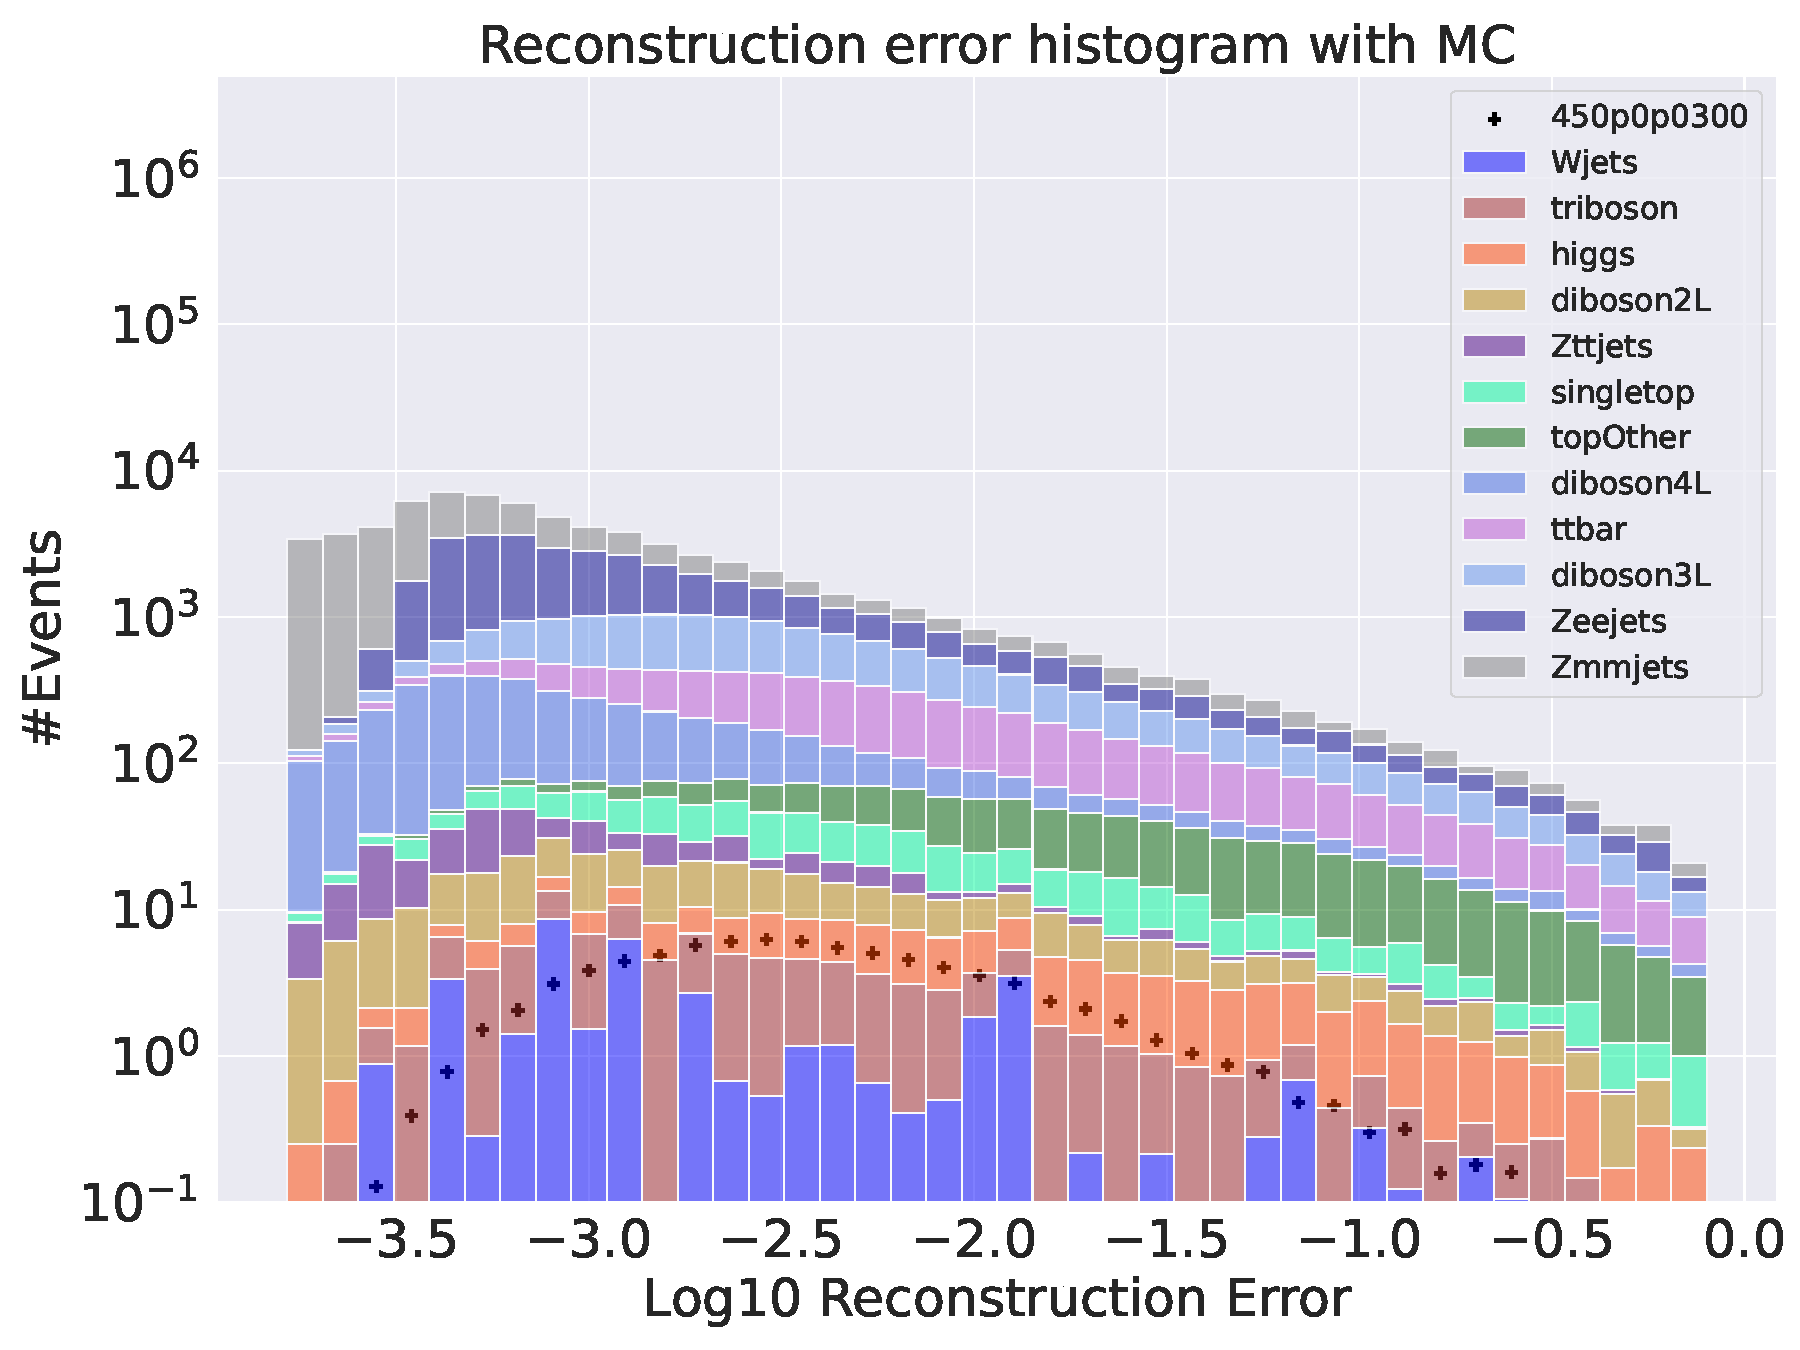
\includegraphics[width=\textwidth]{Figures/AE_testing/big/3lep/b_data_recon_big_rm3_feats_sig_450p0p0300.pdf}
        \caption{ }
        \label{fig:AE_3lep_big_450}
    \end{subfigure}
    \hfill
    \begin{subfigure}{.45\textwidth}
        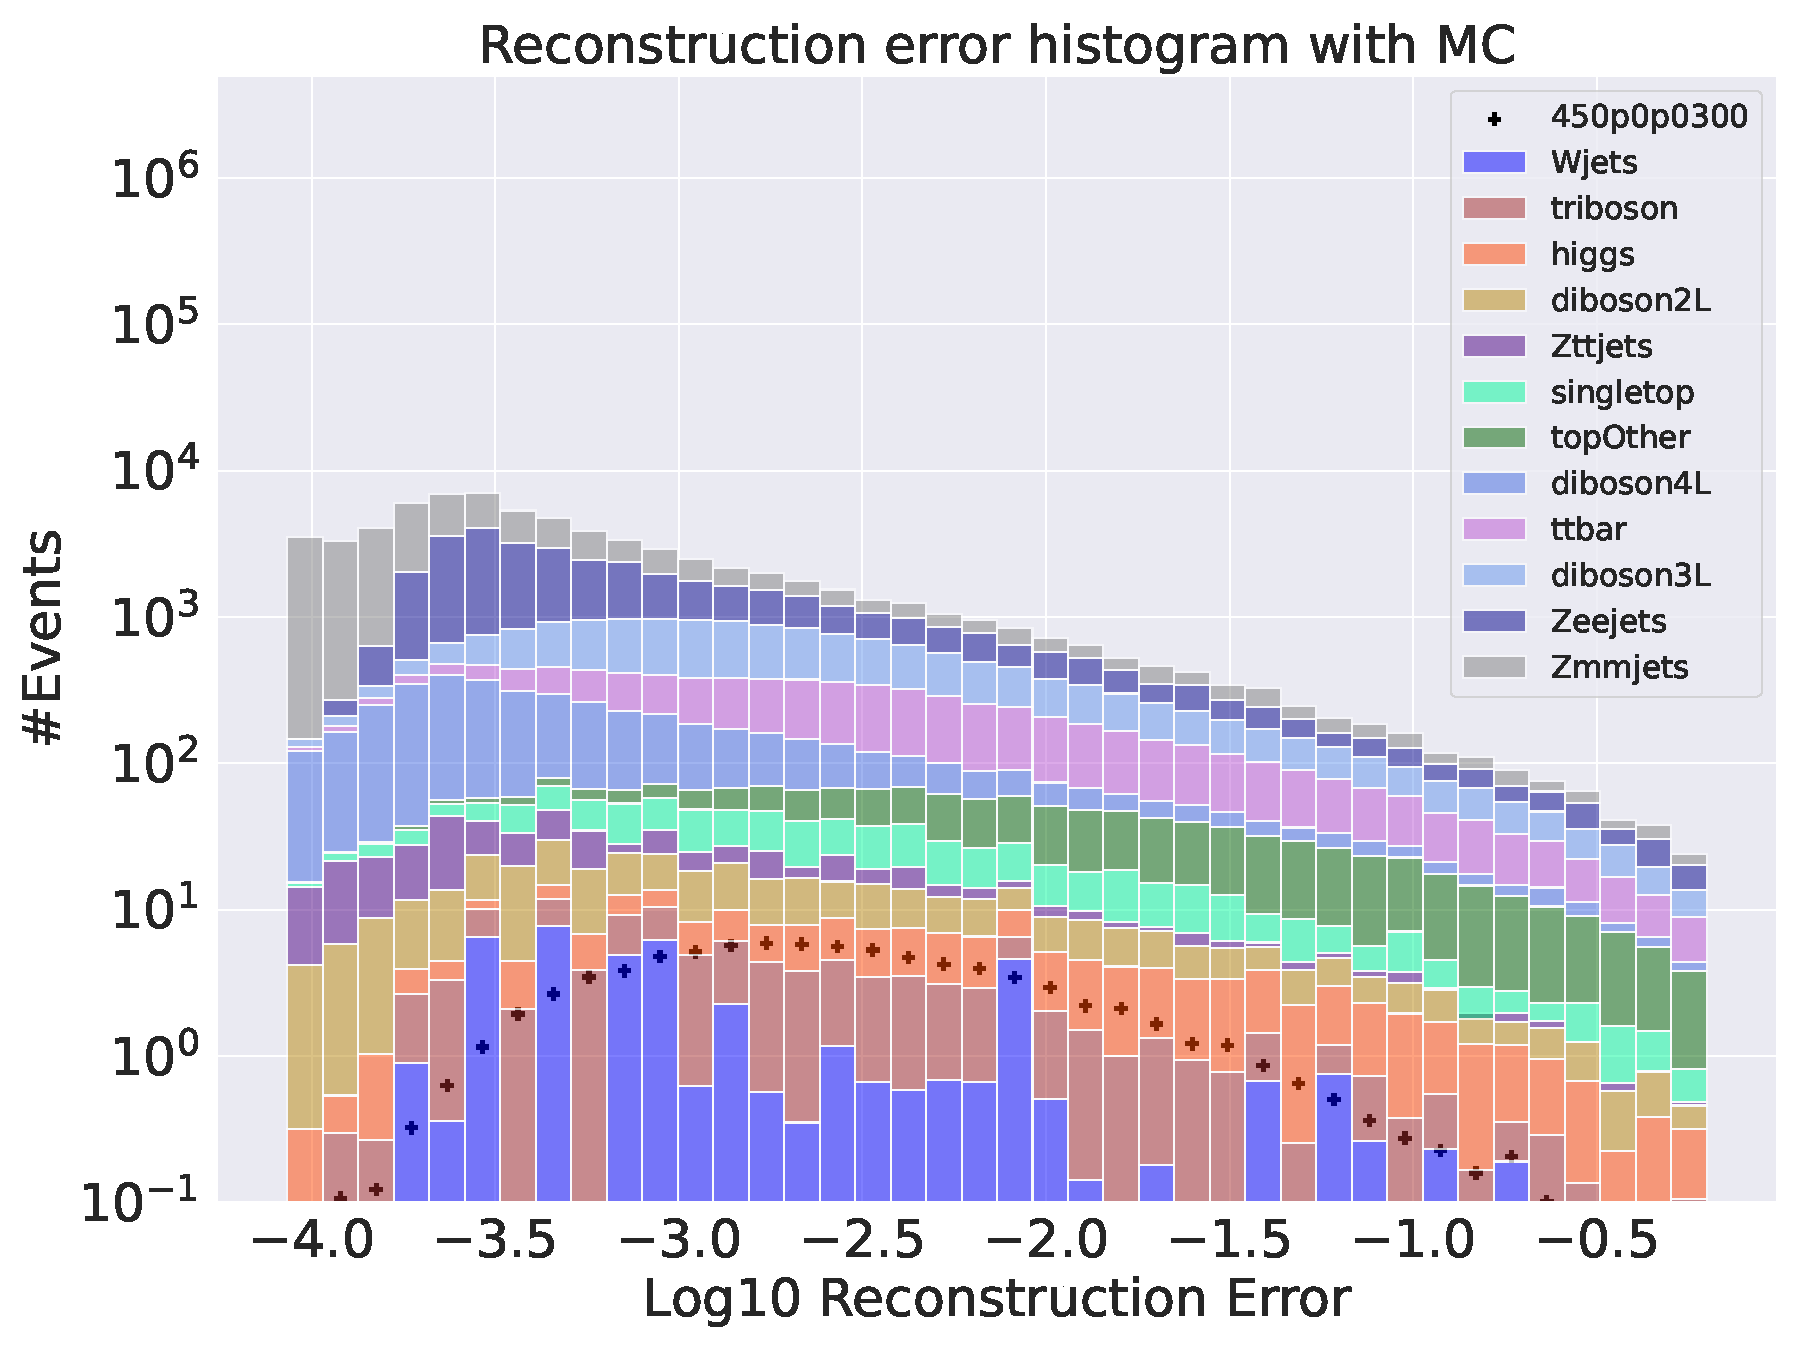
\includegraphics[width=\textwidth]{Figures/AE_testing/small/3lep/b_data_recon_big_rm3_feats_sig_450p0p0300.pdf}
        \caption{}
        \label{fig:AE_3lep_small_450}
    \end{subfigure}
    \hfill
    \begin{subfigure}{.45\textwidth}
        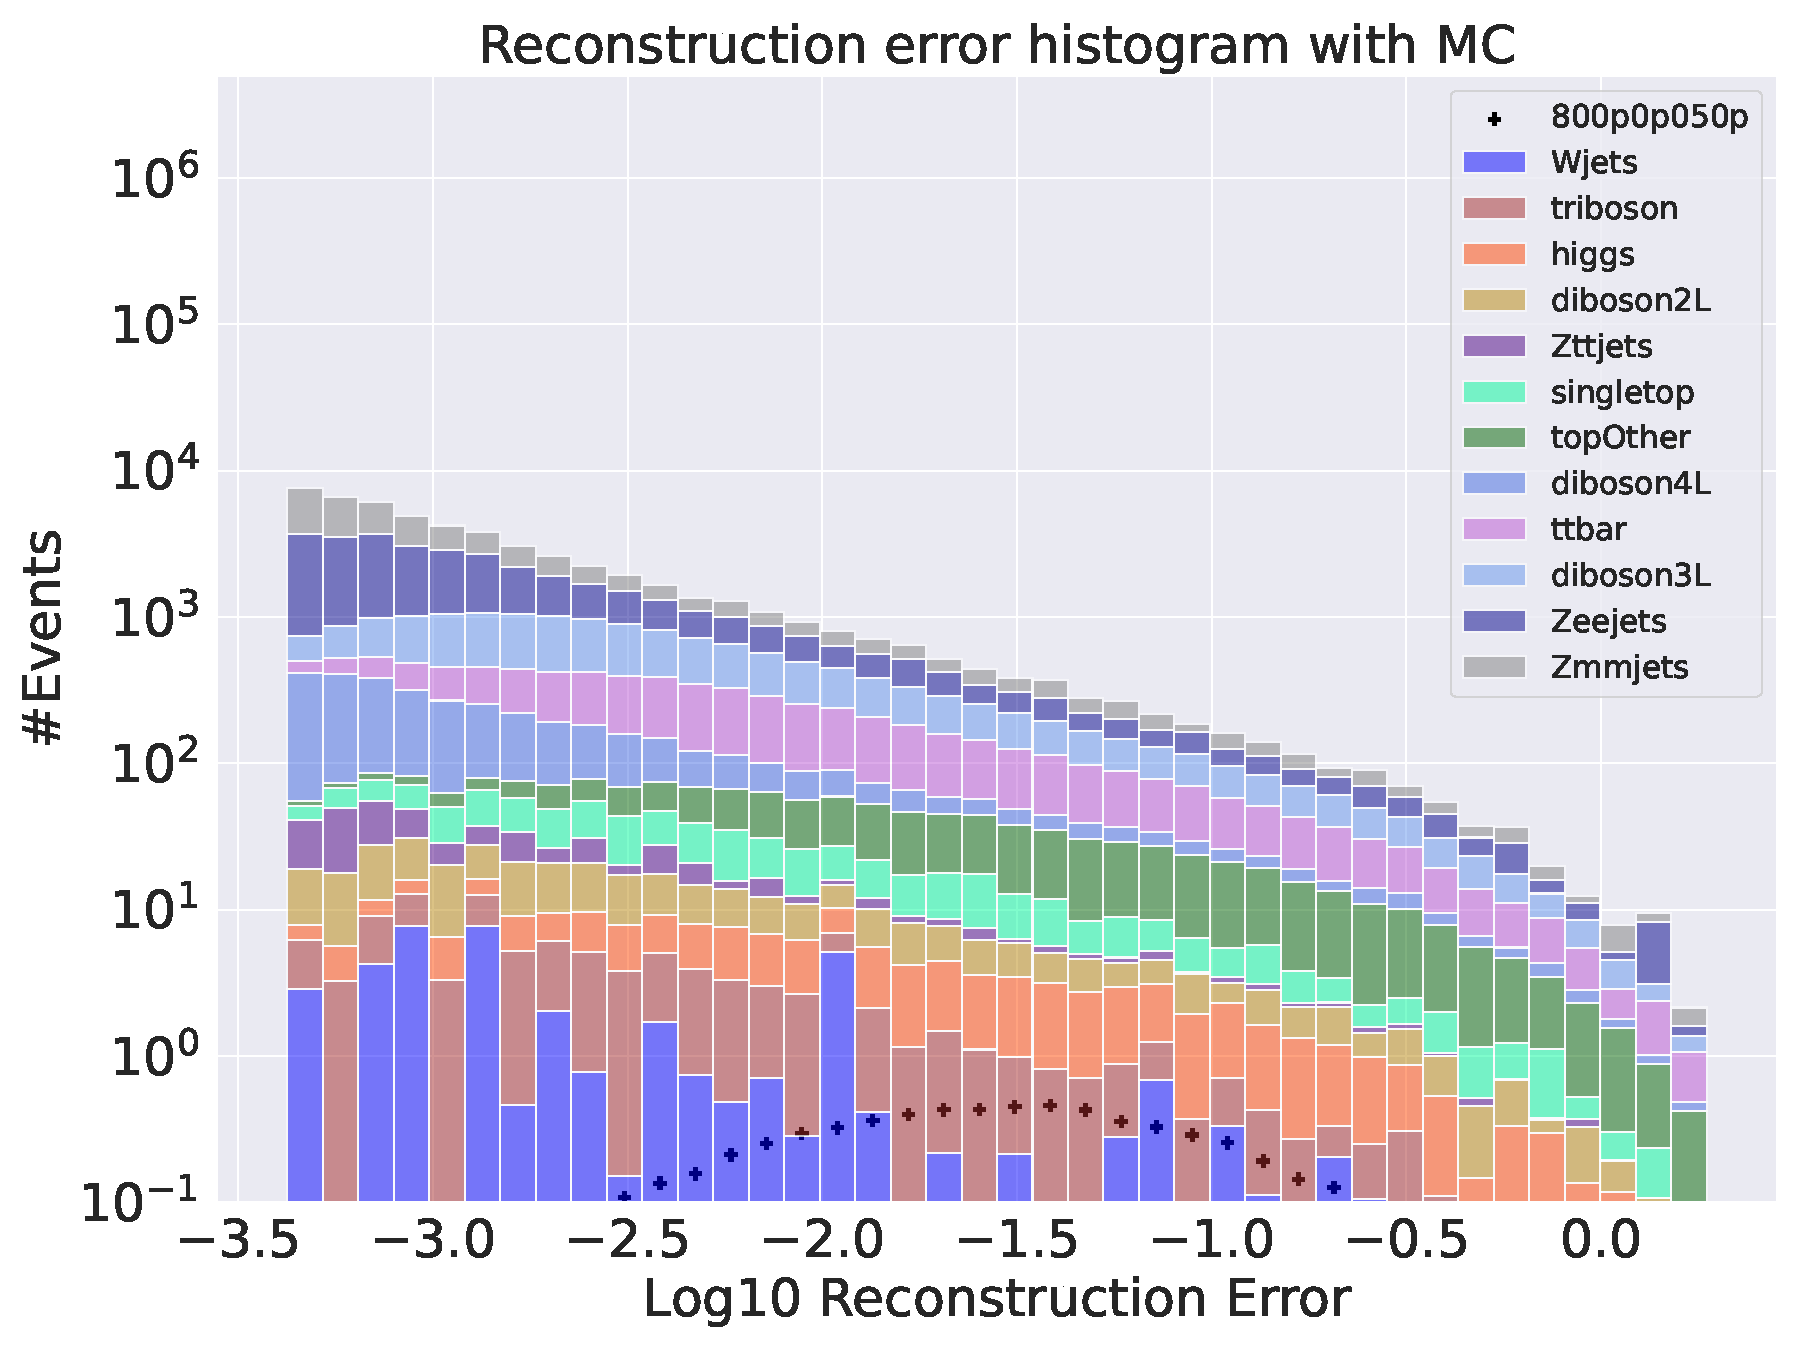
\includegraphics[width=\textwidth]{Figures/AE_testing/big/3lep/b_data_recon_big_rm3_feats_sig_800p0p050p.pdf}
        \caption{}
        \label{fig:AE_3lep_big_800}
    \end{subfigure}
    \hfill   
    \begin{subfigure}{.45\textwidth}
        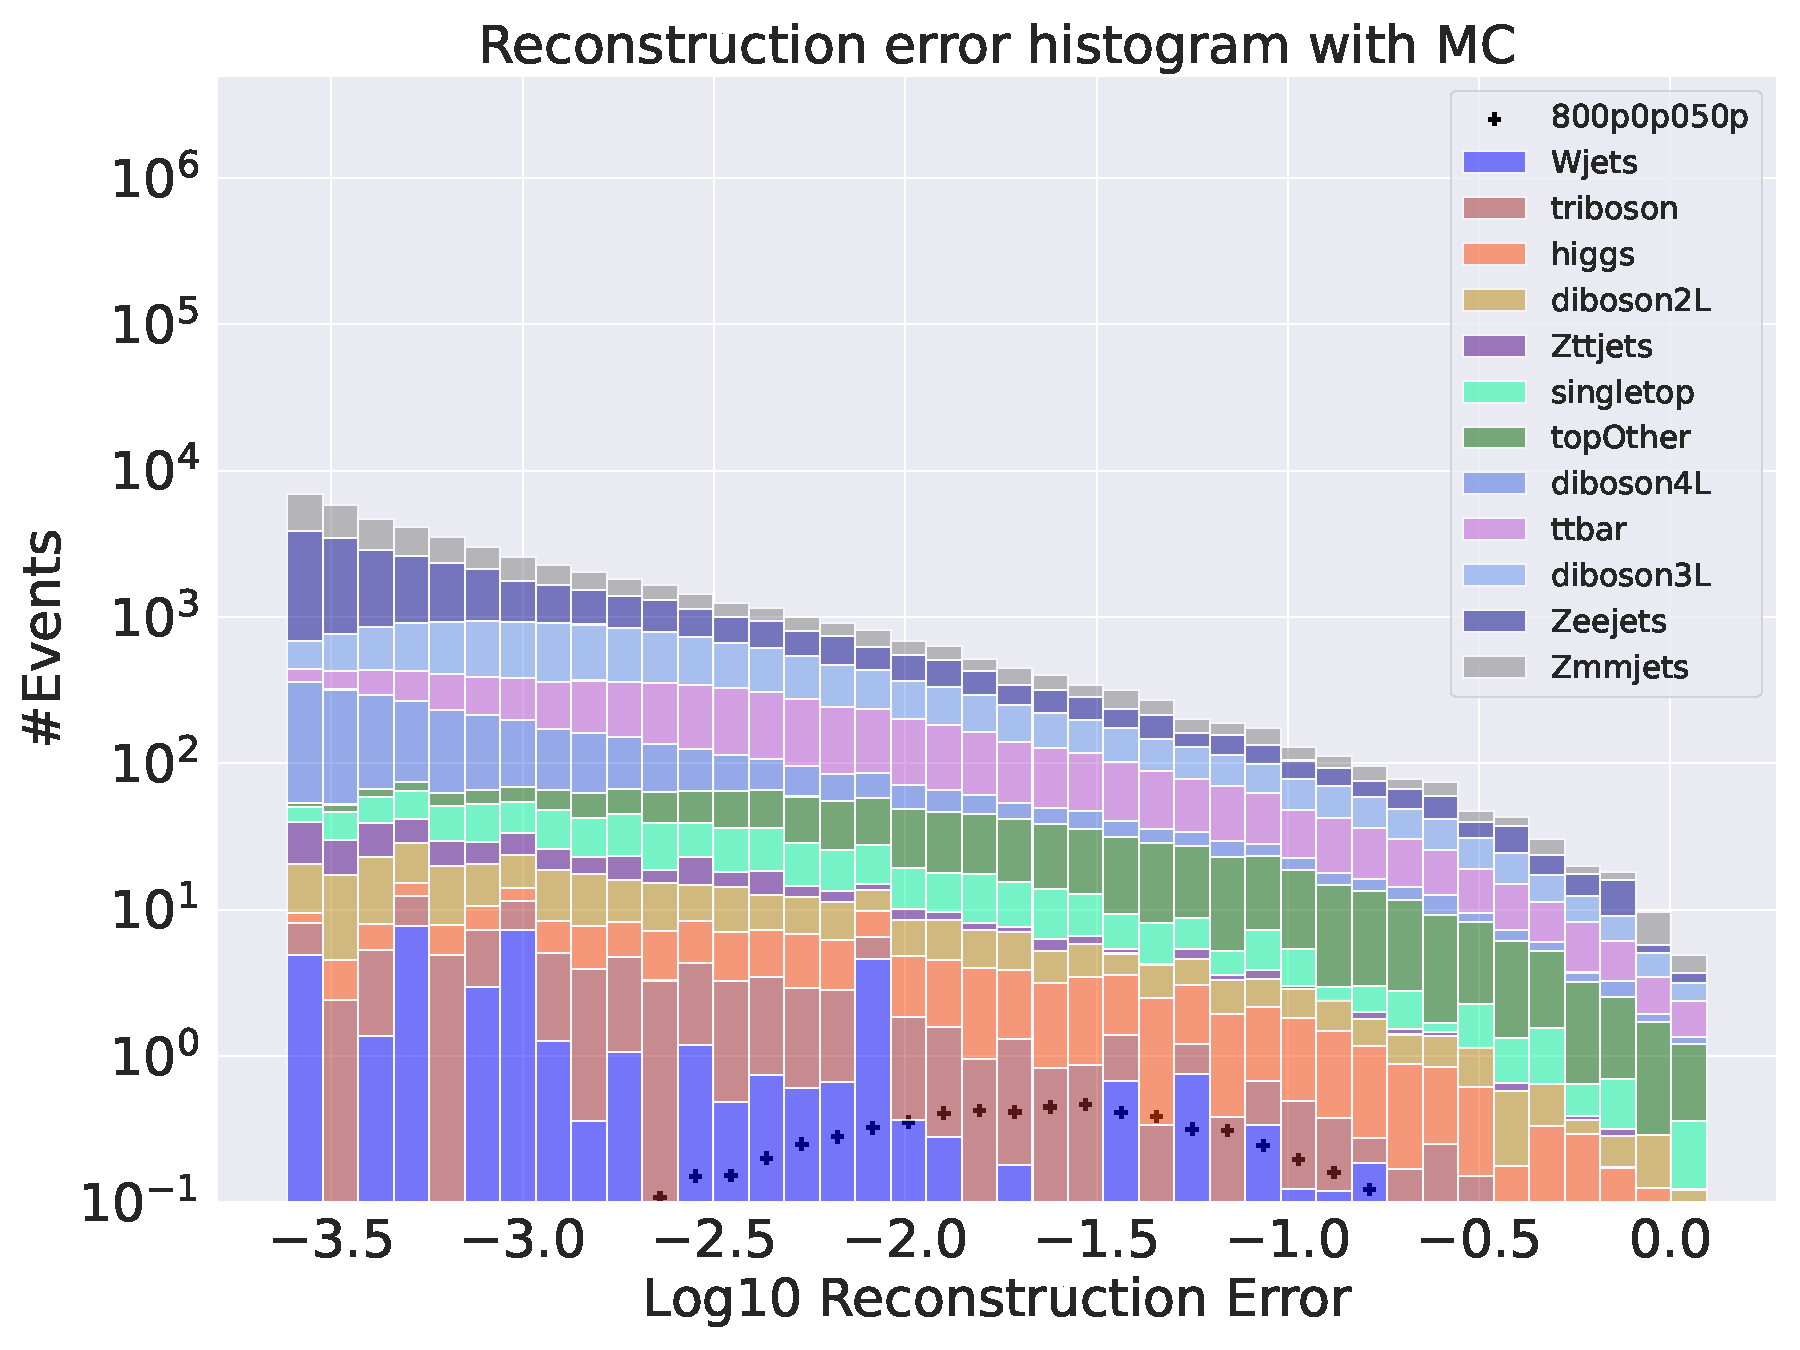
\includegraphics[width=\textwidth]{Figures/AE_testing/small/3lep/b_data_recon_big_rm3_feats_sig_800p0p050p.pdf}
        \caption{}
        \label{fig:AE_3lep_small_800}
    \end{subfigure}
    \hfill      
    \caption[3lep reconstruction error with SUSY signals for AE]{Reconstruction error distribution for the small (left) and large (right)
    regular autoencoder, using the 3 lepton + $e_T^{miss}$ dataset as training and test set. The signals used are 3 lepton + $e_T^{miss}$ 
    finalstate SUSY signals. Figures \ref{fig:AE_3lep_big_450} and \ref{fig:AE_3lep_small_450} shows the SUSY 450 and 300 mass signal, 
    and figures \ref{fig:AE_3lep_big_800} and \ref{fig:AE_3lep_small_800} shows the SUSY 800 and 50 mass signal.}
    \label{fig:AE_3lep_recon_err_both_sig}
\end{figure}


\begin{figure}[H]
    \centering
    \begin{subfigure}{.45\textwidth}
        \includegraphics[width=\textwidth]{}
        \caption{ }
        \label{fig:AE_3lep_big_450_cut_etmiss}
    \end{subfigure}
    \hfill
    \begin{subfigure}{.45\textwidth}
        \includegraphics[width=\textwidth]{}
        \caption{}
        \label{fig:AE_3lep_small_450_cut_etmiss}
    \end{subfigure}
    \hfill
    \begin{subfigure}{.45\textwidth}
        \includegraphics[width=\textwidth]{}
        \caption{}
        \label{fig:AE_3lep_big_800_cut_etmiss}
    \end{subfigure}
    \hfill   
    \begin{subfigure}{.45\textwidth}
        \includegraphics[width=\textwidth]{}
        \caption{}
        \label{fig:AE_3lep_small_800_cut_etmiss}
    \end{subfigure}
    \hfill      
    \caption[$e_T^{miss}$ best cuts for regular autoencoder]{$e_T^{miss}$ distribution for small (left) and large (right) autoencoder.
    Each figure used the best cut of three possibilities, the remainding results are in the appendix. By best, it is meant that the cut
    gave the best significance. Figures \ref{fig:AE_3lep_big_450} and \ref{fig:AE_3lep_small_450} shows the SUSY 450 and 300 mass signal, 
    and figures \ref{fig:AE_3lep_big_800} and \ref{fig:AE_3lep_small_800} shows the SUSY 800 and 50 mass signal.}
    \label{fig:AE_3lep_recon_err_both_sig_cut_etmiss}
\end{figure}

\begin{figure}[H]
    \centering
    \begin{subfigure}{.45\textwidth}
        \includegraphics[width=\textwidth]{}
        \caption{ }
        \label{fig:AE_3lep_big_450_cut_mlll}
    \end{subfigure}
    \hfill
    \begin{subfigure}{.45\textwidth}
        \includegraphics[width=\textwidth]{}
        \caption{}
        \label{fig:AE_3lep_small_450_cut_mlll}
    \end{subfigure}
    \hfill
    \begin{subfigure}{.45\textwidth}
        \includegraphics[width=\textwidth]{}
        \caption{}
        \label{fig:AE_3lep_big_800_cut_mlll}
    \end{subfigure}
    \hfill   
    \begin{subfigure}{.45\textwidth}
        \includegraphics[width=\textwidth]{}
        \caption{}
        \label{fig:AE_3lep_small_800_cut_mlll}
    \end{subfigure}
    \hfill      
    \caption[$m_{lll}$ best cuts for regular autoencoder]{$m_{lll}$ distribution for small (left) and large (right) autoencoder.
    Each figure used the best cut of three possibilities, the remainding results are in the appendix. By best, it is meant that the cut
    gave the best significance. Figures \ref{fig:AE_3lep_big_450} and \ref{fig:AE_3lep_small_450} shows the SUSY 450 and 300 mass signal, 
    and figures \ref{fig:AE_3lep_big_800} and \ref{fig:AE_3lep_small_800} shows the SUSY 800 and 50 mass signal.}
    \label{fig:AE_3lep_recon_err_both_sig_cut_mlll}
\end{figure}



\begin{table}[H]
    \centering
    \caption[Significance table regular autoencoder | 3lep]{Significance table for the regular autoencoder models. For each signal for both the small and 
    large regular autoencoder, the significance is calculated with equation small (left column) and equation large (right column). The 
    reconstruction error cuts used where $[]$ for the SUSY $450p300$ signal and $[]$ for the SUSY 
    $800p50$ signal for the large autoencoder. The reconstruction error cuts used for the small autoencoder where $[]$ 
    for the SUSY $450p300$ signal and $[]$ for the SUSY $800p50$ signal. }
    \label{tab:AE_3lep_significance}
    \begin{tabular}{|llllllll|}
    \hline
    \multicolumn{8}{|c|}{Regular Autoencoder}                                                                                                                                    \\ \hline
    \multicolumn{4}{|c|}{Small}                                                                    & \multicolumn{4}{c|}{Large}                                                  \\ \hline
    \multicolumn{2}{|l|}{450p300}                  & \multicolumn{2}{l|}{800p50}                   & \multicolumn{2}{l|}{450p300}                  & \multicolumn{2}{l|}{800p50} \\ \hline
    \multicolumn{8}{|c|}{Pre reconstruction error cut significance}                                                                                                                           \\ \hline
    \multicolumn{1}{|l|}{} & \multicolumn{1}{l|}{} & \multicolumn{1}{l|}{} & \multicolumn{1}{l|}{} & \multicolumn{1}{l|}{} & \multicolumn{1}{l|}{} & \multicolumn{1}{l|}{}  & \multicolumn{1}{l|}{} \\ \hline
    \multicolumn{8}{|c|}{Post reconstruction error  cut significance}                                                                                                                         \\ \hline
    \multicolumn{1}{|l|}{} & \multicolumn{1}{l|}{} & \multicolumn{1}{l|}{} & \multicolumn{1}{l|}{} & \multicolumn{1}{l|}{} & \multicolumn{1}{l|}{} & \multicolumn{1}{l|}{}   & \multicolumn{1}{l|}{}  \\ \hline
    \multicolumn{1}{|l|}{} & \multicolumn{1}{l|}{} & \multicolumn{1}{l|}{} & \multicolumn{1}{l|}{} & \multicolumn{1}{l|}{} & \multicolumn{1}{l|}{} & \multicolumn{1}{l|}{}   & \multicolumn{1}{l|}{}  \\ \hline
    \multicolumn{1}{|l|}{} & \multicolumn{1}{l|}{} & \multicolumn{1}{l|}{} & \multicolumn{1}{l|}{} & \multicolumn{1}{l|}{} & \multicolumn{1}{l|}{} & \multicolumn{1}{l|}{}   & \multicolumn{1}{l|}{} \\ \hline
    \end{tabular}
\end{table}